%#!simpdftex relativita.tex
\chapter{Meccanica relativistica}
\minitoc 
In questo capitolo ci interessiamo alla
generalizzazione relativistica di velocit\`a,
accelerazione\index{accelerazione!non relativistica}, impulso e
forza. Vogliamo che tutti gli oggetti con cui si entri in contatto
siano parte dello spazio di Minkowski, sicch\'e trasformino
correttamente da un sistema inerziale ad un altro, ossia
soddisfino il principio di relativit\`a\footnote{Questo vuol dire che se
in un sistema di riferimento $F = ma$, allora in un altro sistema di
riferimento, che si pu\`o ottenere mediante una trasformazione di
Lorentz, varr\`a la relazione $F' = m' a' $}. 

Questo significa che vogliamo definire delle grandezze che si comportino
in tale modo: sia $\bef{F}$ la forza in un sistema $S$, e \(\bef{p}\)
l'impulso; in un sistema $S'$ la forza sar\`a $\bef{F'}$, e l'impulso
\(\bef{p'}\); si passer\`a dagli uni agli altri con una trasformazione di
Lorentz, ossia:
\begin{displaymath}
\bef{F}' = \la \bef{F}, 
\end{displaymath}
\begin{displaymath}
 \bef{p}' = \la \bef{p}, 
\end{displaymath}
in modo che l'equazione \(\bef{F}= \de \bef{p} / \de t\) sia la medesima
per entrambi i sistemi di riferimento, in accordo con il principio di
relativit\`a. In pratica stiamo cercando delle leggi covarianti.

Inoltre, ci preme che per $\beta<<1$, si ritrovino le quantit\`a 
classiche. Non ci cureremo per\`o di dimostrarlo, lasciandolo come facile
esercizio a cura del lettore. Ci interessa poi addentrarci nella
dinamica dei processi tra particelle, cosa di cui ci occuperemo
nell'ultima parte del capitolo.
\section{ Grandezze fondamentali}
\begin{osservazione} In cinematica non relativistica si ha:
\begin{displaymath}
 \mathbf{x}(t),\quad
 \mathbf{v}(t)=\frac{\rem{d}\mathbf{x}(t)}{\rem{d}t},\quad
 \mathbf{a}(t)=\frac{\rem{d}\mathbf{v}(t)}{\rem{d}t}
\end{displaymath}
$\mathbf{x}(t)$ \`e un vettore tuttavia: come gi\`a detto noi
vogliamo un quadrivettore. Allora:%
\footnote{\(x^\mu\), non \`e propriamente un quadrivettore, poich\'e
 sotto
una trasformazione di Poincar\'e esso diviene
 $x'^{\mu}=\la^{\mu}{}_{\nu}x^{\nu}+a^{\nu}$, ma si ovvia 
prendendone il dif\mbox{}ferenziale, ovvero
 $\rem{d}x'^{\mu}=\la^{\mu}{}_{\nu}\rem{d}x^{\nu}$.}
\begin{equation}
 \mathbf{x}\rightarrow x^{\mu}
\end{equation}
\begin{equation}
 t\rightarrow\tau \quad\mbox{ tempo proprio.}
\end{equation}
Perch\'e vogliamo usare il tempo proprio e non il tempo? La risposta sta
 nella definizione di tempo proprio (\(\de \tau = \de s /c\)): essa
 permette allo stesso di essere indipendente dal sistema di riferimento,
 al contrario di \(t\): dunque parametrizzare i moti con il tempo
 proprio, e non con il tempo, permette di ottenere un parametro che sia
 indipendente dal sistema di riferimento, e che sia quindi covariante.

 La scelta naturale cade tuttavia sulla radice di $\de s^2=\de
x^{\nu}g_{\mu\nu}\de x^{\mu}$ (solo nel caso che non si abbia a che fare
con particelle con velocit\`a pari a $c$). Per questo il lettore abbia
la cura di mostrare la validit\`a della seguente relazione (che discende
da \(\de s^2 = \de x^{\mu}\de x_{\mu}\)):
\begin{equation}
 \D s=\D t\, \frac{c}{\gamma}
\end{equation}
che ci torner\`a molto utile in seguito. Facciamo subito notare che,
 dacch\'e $\de s^2$ \`e l'intervallo spazio temporale del moto, la $v$
 all'interno di $\gamma$ \`e la velocit\`a a cui avviene il moto.
\end{osservazione}
\begin{definizione}[La quadrivelocit\`a]
\index{quadrivelocit\`a} Possiamo a questo punto prendere l'analogo
della velocit\`a:
\begin{equation}
 \mathbf{v}(t)\rightarrow \frac{\D x^{\mu}}{\D s}=\frac{\D
x^{\mu}}{c\D t}\gamma  \mbox{\scriptsize(\`e un quadrivettore,
in quanto rapporto di un quadrivettore con uno scalare ).}
\end{equation}
Si ottiene:
\begin{equation}
 u^0=\frac{\D x^0}{\D s}=\gamma,
\end{equation}
\begin{equation}
 u^i=\frac{\D x^i}{\D s}=\frac{\gamma}{c}\frac{\D x^i}{\D t};
\end{equation}
dunque, in def\mbox{}initiva, si ha:
\begin{equation}
 u^{\mu}=\left(\gamma,\frac{\gamma}{c}\mathbf{v}\right)
\end{equation}
Notiamo poi che dalla def\mbox{}inizione segue che:
\begin{equation}
 u^{\mu}u_{\mu}=1\label{eq:uperu}
\end{equation}
\begin{equation}
 \mbox{\scriptsize(al lettore i calcoli)}
\end{equation}
\end{definizione}
\begin{definizione}[La quadriaccelerazione]
\index{quadriaccelerazione} Come prima abbiamo introdotto la
quadrivelocit\`a come la derivata temporale del vettore posizione,
ora introduciamo la quadriaccelerazione come la derivata temporale
della quadrivelocit\`a:
\begin{displaymath}
 \mathbf{a}=\frac{\D \mathbf{v}}{\D t}=\frac{\D^2 \mathbf{x}}{\D
t^2}\rightarrow w^{\mu}=\frac{\D u^{\mu}}{\D s}.
\end{displaymath}
Ricaviamone le componenti (si usa qui il fatto che $\frac{\D
\gamma}{\D t}=\frac{\gamma^3}{c^2}\mathbf{v}\cdot\mathbf{a}$,
relazione che si ottiene derivando appunto $\gamma$ rispetto al
tempo, ricordando che $\mathbf{v}=\mathbf{v}(t)$):
\begin{displaymath}
 w^0=\frac{\D u^0}{\D s}=\frac{\gamma}{c}\frac{\D \gamma}{\D
t}=\frac{\gamma^4}{c^3}\mathbf{v}\cdot\mathbf{a},
\end{displaymath}
\begin{equation}
 w^i=\frac{\D u^i}{\D s}=\frac{\gamma}{c^2} 
\frac{\D (\gamma v^i)}{\D t} 
  =
  \frac{\gamma^2}{c^2}a^i + 
  \frac{\gamma^4}{c^4}(\mathbf{v}\cdot\mathbf{a})v^i; 
\end{equation}
prendiamo ora la (\ref{eq:uperu}), e deriviamola rispetto a $s$.
Ne esce:
\begin{equation}
w\cdot u=0 \label{eq:perpendicolari}
\end{equation}
il che implica che quadri-velocit\`a e quadri-accelerazione sono tra loro
ortogonali (sempre!).
\end{definizione}
\begin{definizione}[Il quadrimpulso]
\index{quadrimpulso}Si generalizza ora l'idea di impulso:
\begin{equation}
 \mathbf{p}=m\mathbf{v}\rightarrow p^{\mu}:=mcu^{\mu}
\end{equation}
Dunque il quadrimpulso risulta:
\begin{equation}
 p^{\mu} = 
  \left(\frac{mc}{\sq},\frac{m\mathbf{v}}{\sq}\right)\label{eq:quadrimpulso}
\end{equation}
Viene ora spontaneo interrogarsi su $mc\gamma$, il primo termine
del quadrimpulso: esso infatti \`e $\frac{E}{c}$. Cosa c'\`e di
strano? Prendiamo il caso $\beta<<1$. Non \`e
dif\mbox{}f\mbox{}icile vedere che:
\begin{equation}
 cp^0=mc^2\gamma \stackrel{\beta<<1}{\simeq}mc^2+\frac{1}{2}mc^2
\frac{v^2}{c^2}=mc^2+\frac{1}{2}mv^2
\end{equation}
Ora, se $\frac{1}{2}mv^2$ \`e chiaramente l'energia cinetica, non
si ha un analogo classico per il termine~$mc^2$,
\index{energia!massa@$mc^2$}in quanto da ci\`o che s'\`e appena
scritto, risulta che un corpo in quiete, per il solo fatto di
avere massa, ha un'energia pari a~$mc^2$. Saremmo tentati di
definire l'energia come $cp^0-mc^2$, ma questo oggetto non
trasforma come un tensore, e viola il principio di relativit\`a.
Osserviamo ora che:
\begin{equation}
p^{\mu}p_{\mu}=\frac{E^2}{c^2}-\mathbf{p}\;{}^{2} =
\frac{m^2c^2}{1-v^2/c^2}-\frac{m^2v^2}{1-v^2/c^2}=m^2c^2
\label{eq:masshell}\end{equation}\index{equazione!mass shell}
Questa relazione vive anche se un corpo ha velocit\`a della luce
(e quindi massa nulla), e si scrive come $E=c|\mathbf{p}|$.
\end{definizione}
\section{ La quadriforza}
\begin{osservazione}[Particella non soggetta a forze] Se una particella \`e in
moto nello spazio di Minkowski, essa \`e soggetta alle equazioni
\begin{equation}
 \frac{\de p^{\mu}}{\de s}=0\qquad\mbox{e }p^{\mu}p_{\mu}=m^2c^2,
\end{equation}
sempre che si sia in assenza di forze. Nel caso di una particella
di massa nulla, non potendo parametrizzare con $\de s$, in quanto
esso \`e sempre pari a 0, parametrizzeremo con un parametro
scalare $\zeta$; pi\`u precisamente:
\begin{equation}
 \frac{\de^2x^{\mu}}{\de \zeta^2}=0,\quad \mbox{ con } ds=0
\end{equation}
\end{osservazione}
\begin{definizione}[La quadriforza]
\index{quadriforza} Se una particella \`e invece soggetta a forze
esterne, vive la seguente relazione:
\begin{equation} \frac{\de p^{\mu}}{\de s}=\mt{F}^{\mu}
\label{eq:covariantem}
\end{equation}
\begin{center}
\scriptsize Equazione covariante di Minkowski\index{equazione!di
Minkowski}\index{Minkowski!equazione di}
\end{center}
Nel caso si voglia trovare esplicitamente i termini di $\mt{F}$,
deriviamo rispetto a~$s$ la~(\ref{eq:quadrimpulso}), ottenendo:
\begin{equation}
 \mt{F}^{\mu}=\left(\frac{\gamma}{c^2}\frac{\de E}{\de
t},\frac{\gamma}{c}\frac{\de \mathbf{p}}{\de t}\right)
\end{equation}
Ma $\de \mathbf{p}/ \de t$ non \`e altro che la $\mathbf{F}$ della
meccanica pre-relativistica, e inoltre, dacch\'e sussiste la legge
della potenza, si ha che vive la relazione $\frac{\de E}{\de
t}=\mathbf{F}\cdot\mathbf{v}$. Questo semplif\mbox{}ica un po' le
cose, permettendo di scrivere:
\begin{equation}
\mt{F}^{\mu}=\frac{\gamma}{c}
\left(\frac{1}{c}\mathbf{F}\cdot\mathbf{v}, \mathbf{F}\right).
\end{equation}
Analogamente alla (\ref{eq:perpendicolari}) si trova:
\begin{equation}
 \mt{F}^{\mu}u_{\mu} = \mt{F}^0 - 
  \frac{\mathbf{\mt{F}}\cdot\mathbf{v}}{c}=0
\end{equation}
Da qui \`e possibile vedere che $\mt{F}^{\mu}$ non \`e
indipendente da $\mathbf{v}$, cosa che prima accadeva.
\end{definizione}
\section{ Sistemi di riferimento}
Nei fenomeni in cui si ha a che fare con particelle che
interagiscono a velocit\`a prossime a quelle della luce, si rende
indispensabile la meccanica relativistica, poich\'e essa
descrive in maniera corretta le quantit\`a in gioco.
Questo spiega il larghissimo uso che se ne fa in
fisica nucleare e sub-nucleare. In questa sezione
affronteremo decadimento di particelle e urti tra
particelle.

%\vspace{0.5cm}

Per quanto riguarda la nostra analisi di urti e decadimento,
prenderemo in considerazione due sistemi di riferimento, il
sistema di riferimento del centro di massa, $\cem$, e il sistema
di riferimento del laboratorio, $\lab$\footnote{ Per capirci: in
$\cem$ il centro di massa del sistema \`e fermo, mentre $\lab$ \`e
il sistema che non \`e propriamente quello del laboratorio, ma un
altro sistema che risulta a noi comodo per descrivere i fenomeni
che studiamo}. Facciamo un esempio per impratichirsi un po' con
questi due sistemi;

\begin{esempio} Mettiamoci in $\lab$, e consideriamo due particelle, la prima
che si muove lungo l'asse $x$ con quantit\`a di moto
$\mathbf{p}_1=p$, e la seconda, ferma, per la quale vale dunque la
relazione $\mathbf{p}_2=0$. Perci\`o la sua energia \`e (sia $c=1$
in tutti i conti che facciamo in questo esempio) $E_2=m_2$. Si ha
poi:
\begin{equation}
 p_1=(E_1,p,0,0)
\end{equation}
\begin{equation}
 p_2=(m_2,0,0,0)
\end{equation}
\begin{equation}
E_1=\sqrt{p^2+m_1^2}.\label{eq:energiaur}
\end{equation}
In $\cem$ si ha invece che la quantit\`a di moto totale \`e nulla,
e dunque:\footnote{Introduciamo ora la seguente notazione: ogni
quantit\`a contrassegnata da $\star$, verr\`a intesa come
calcolata nel centro di massa, indipendentemente dal fatto che
$\star$ \ sia posizionata in alto o in basso (ovvero
$p^{\star}=p_{\star}$), per questioni di comodit\`a.}
$$
\mathbf{p}_1^{\star}+\mathbf{p}_2^{\star}=0
$$
il che porge:
$$
|\mathbf{p}_1^{\star}|=|\mathbf{p}_2^{\star}|=p^{\star}
$$
Dunque:
$$
p_1^{\star}=(E_1^{\star},p^{\star},0,0)
$$
$$
p_2^{\star}=(E_2^{\star},-p^{\star},0,0)
$$
Per passare da $\lab$ a $\cem$ si effettua una trasformazione di
Lorentz lungo $x$. Prima di farlo introduciamo tuttavia le
quantit\`a $p_{\rem{tot}}$ e $p_{\rem{tot}}^{\star}$, cos\`i
definite:
$$
p_{\rem{tot}}=p_1+p_2=(E_1+m_2,p,0,0)
$$
$$
p_{\rem{tot}}^{\star}=p_1^{\star}+p_2^{\star}=(E_1^{\star}+E_2^{\star},0,0,0)
$$
Applicando le trasformazioni di Lorentz lungo $x$ otteniamo:
\begin{equation}
(p_{\rem{tot}}^{\star})_x=\gamma_{\rem{CM}}[(p_{\rem{tot}})_x -
\beta_{\rem{CM}}p_{\rem{tot}}^{0}] \label{eq:lorenzx}
\end{equation}
Ricordando che $c=1$, si ha che $\beta_{\rem{CM}}=\rem{v}$
($\rem{v}$ \`e la velocit\`a di $\cem$ rispetto a $\lab$), e
la~(\ref{eq:lorenzx}) porge:
$$
(p_{\rem{tot}}^{\star})_x = 0
=\gamma_{\rem{CM}}[p-\beta_{\rem{CM}}(E_1+m_2)],
$$
che a sua volta d\`a:
$$
\beta_{\rem{CM}}=\frac{p}{E_1+m_2}.
$$
Dacch\'e $p=m_1\gamma_{v_1}v_1$, usando la (\ref{eq:energiaur}),
si trova $E_1=m_1\gamma_{v_1}$, dalle quali:
$$
\beta_{\rem{CM}}=\frac{m_1\gamma_{v_1}v_1}{m_1\gamma_{v_1}+m_2}=\rem{v} 
$$
Volendo esprimere~$\beta_{\rem{CM}}$ in un'altra forma, usiamo le
trasformazioni di Lorentz lungo~$z$ per la particella~2,
ottenendo:
$$
0=\gamma_{\rem{CM}}(-p^{\star}+\beta_{\rem{CM}}E_2^{\star})
$$
Con qualche semplice passaggio si arriva a:
\begin{equation}
\beta_{\rem{CM}}=\frac{p^{\star}}{E^{\star}_2}=v_2^{\star}.
\label{eq:beta}
\end{equation}
Questo risultato era da aspettarsi, in quanto per annullare la
velocit\`a della particella ferma in~$\lab$, velocit\`a che
in~$\cem$ vale~$v_2^{\star}$, \`e necessaria una trasformazione
che abbia $\beta_{\rem{CM}}=v_2^{\star}$.
\end{esempio}
\section{ Processi tra particelle (dinamica relativistica)}
\subsection{ Decadimento}\index{decadimento}
Dopo esserci impratichiti\footnote{Si spera!} con i nuovi sistemi
di riferimento che useremo nelle nostre analisi, affrontiamo pi\`u
approfonditamente il fenomeno del decadimento. il quale consiste
nel processo che, da un particella iniziale con massa $M$,
restituisce $n$ particelle separate $m_1\ldots m_n$, come in
figura \vref{fig:decadimento}.

\setlength{\unitlength}{1mm}

\begin{figure}[htbp]
\begin{center}
\begin{picture}(80,50)
\put(0,0){\framebox(80,50)}
\put(5,25){\vector(1,0){40}}\put(25,27){$M$}\put(45,25){\vector(1,1){20}}
\put(45,25){\vector(1,-1){20}} \put(45,25){\vector(2,1){24}}
\put(50,37){$m_1$}\put(50,12){$m_n$} \put(45,25){\line(3,-2){4}}
\put(51,21){\line(3,-2){4}}\put(57,17){\line(3,-2){4}}
\put(63,13){\vector(3,-2){5}} \put(60,30){$m_2$}
\end{picture}
\end{center}
\caption{Decadimento di una generica particella con massa
$M$}\label{fig:decadimento}
\end{figure}

Ci si aspetterebbe, abbastanza intuitivamente, che
$m_1+\ldots+m_n=M$; invece ci\`o non accade, poich\'e ci\`o che si
conserva \`e il quadrimpulso \index{quadrimpulso!conservazione
del}, nel caso si sia in assenza di forze esterne. La prima
domanda che viene spontaneo chiedersi \`e, date le masse delle
particelle, quali sono le condizione affinch\'e avvenga il
decadimento. Se siamo nel sistema di riferimento del centro di
massa, vale la seguente relazione:
$$
\frac{E^{\star}}{c}=Mc=\sum_{i=1}^{n}\frac{E^{\star}_{i}}{c}.
$$
Si vede subito che:
$$
\sum_{i=1}^{n}\frac{E^{\star}_{i}}{c}\geq\sum_{i=1}^{n}m_{i}c$$
$$\Longrightarrow$$
\begin{equation}
\fbox{$\displaystyle M\geq\sum_{i=1}^{n}m_{i}$}
\label{eq:decadimento}
\end{equation}
La (\ref{eq:decadimento}) \`e dunque la condizione per avere il
decadimento della particella~$M$ in~$n$ particelle.
\subsection{ Decadimento a due corpi}
Consideriamo ora il decadimento a due corpi, ovvero $M\rightarrow
m_{1}+m_{2}$. In questo caso in $\cem$, $E_{1}^{\star}$ ed
 $E_{2}^{\star}$, sono completamente determinate. Vive la
relazione:
$$
\mathbf{p}^{\star}_{1}+\mathbf{p}^{\star}_{2}=0\Rightarrow
|\mathbf{p}^{\star}_{1}|=|\mathbf{p}^{\star}_{2}|=p^{\star}\Rightarrow
\mathbf{p}^{\star}_{1}\cdot\mathbf{p}^{\star}_{2}=-p_{\star}^2
$$
Il fatto che $|\mathbf{p}^{\star}_{1}|=|\mathbf{p}^{\star}_{2}|$
comporta che:
\begin{equation}
(p_1^{\star})^2=(E^{\star}_{1})^2-m^2_1c^2=(E^{\star}_{2})^2-m^2_2c^2=(p_2^{\star})^2
\label{eq:endec1}
\end{equation}
Per la legge di conservazione dell'energia si ha:
\begin{equation}E^{\star}_{1}+E^{\star}_{2}=Mc^2.\label{eq:nuova}\end{equation}
Dividendo membro a membro le ultime due equazioni, tramite
semplici passaggi si giunge~a:
\begin{equation}
E^{\star}_{1}-E^{\star}_{2}=\frac{m^2_1-m^2_2}{M}.
\label{eq:endec2}
\end{equation}
A questo punto una semplice manipolazione algebrica della
(\ref{eq:nuova}) e della (\ref{eq:endec2}) ci porta a:
\begin{equation}
E^{\star}_{1}=c^2\frac{M^2+m^2_1-m^2_2}{2M} \label{eq:endecfin1}
\end{equation}
\begin{equation}
E^{\star}_{2}=c^2\frac{M^2-m^2_1+m^2_2}{2M} \label{eq:endecfin2}
\end{equation}
\begin{equation}
(\frac{E^{\star}_{1}}{c} - m_1^2
c^2)=p^2_{\star}=c^2\frac{M^4+m_{1}^4+m_{2}^4-2m_{1}^2m_{2}^2-2(m_{1}^2+m_{2}^2)M^2}{4M^2}
\end{equation}
Osserviamo che nel decadimento tra particelle, l'angolo
$\vartheta^{\star}$ della figura \vref{fig:decaincm} non \`e
determinato.

\begin{figure}[htbp]
\begin{center}
\begin{picture}(80,50)
\put(0,0){\framebox(80,50)}
\put(5,25){\line(1,0){4}}\put(12,25){\line(1,0){4}}\put(20,25){\line(1,0){4}}
\put(28,25){\line(1,0){4}}\put(36,25){\line(1,0){4}}\put(44,25){\line(1,0){4}}
\put(40,25){\vector(3,1){15}}\put(40,25){\vector(-3,-1){15}}\qbezier(53,25)(54,28)(52,29)
\qbezier(44,25)(40,22)(34,23)\put(48,31){$m_1$}\put(28,17){$m_2$}
\put(57,27){$\vartheta_1=\vartheta_{\star}$}
\put(40,19){$\vartheta_2=\pi-\vartheta_{\star}$}
\put(52,25){\line(1,0){4}}\put(60,25){\line(1,0){4}}\put(68,25){\line(1,0){4}}
\end{picture}
\end{center}
\caption{Decadimento a due corpi in $\cem$}\label{fig:decaincm}
\end{figure}

Esaminiamo per\`o il decadimento nel sistema laboratorio, il quale
si muove con velocit\`a~$-\mathbf{v}$ rispetto alla particella che
decade, ovvero rispetto a $\cem$. Le cose vanno come in
f\mbox{}igura~\ref{fig:decainlab}

\begin{figure}[htbp]
\begin{center}
\begin{picture}(80,50)

\put(5,38){\vector(0,1){6}}\put(5,38){\vector(1,0){6}}
\put(9,36){\scriptsize$x$} \put(3,42){\scriptsize$y$}
\put(0,0){\framebox(80,50)}
\put(5,25){\vector(1,0){40}}\put(25,27){$M$}\put(45,25){\vector(1,1){20}}
\put(45,25){\vector(1,-1){20}}
\put(50,37){$m_1$}\put(50,12){$m_n$}\multiput(45,25)(6,0){4}{\line(1,0){4}}
\put(53,27){$\vartheta_1$}\put(53,21){$\vartheta_2$}
\qbezier(51,25)(52,27)(50,30)\qbezier(52,25)(52,23)(50,20)\end{picture}
\end{center}
\caption{Decadimento a due corpi in $\lab$}\label{fig:decainlab}
\end{figure}

Possiamo dunque usare le trasformazioni di Lorentz, usando gli
assi come in f\mbox{}igura \vref{fig:decainlab}, in particolare
con l'asse $x$ posto lungo la traiettoria della particella con
massa $M$, e $z$ orientato coerentemente. Usiamo poi $\alpha=1,2$
per indicare la particella 1, o la particella 2. Trasformiamo
dunque $p^{\mu}=(E,\mathbf{p})$ lungo l'asse $x$. In $\cem$ si ha:
$$
p_{\alpha x}^{\star}=p^{\star}\cos\vartheta_{\alpha}^{\star}
$$
$$
p_{\alpha y}^{\star}=p^{\star}\sin\vartheta_{\alpha}^{\star}
$$
Dacch\'e l'energia si trasforma come il tempo, avremo:
$$
E_{\alpha}=\gamma(E_{\alpha}^{\star}+v\,p_{\alpha
x}^{\star})=\gamma(E_{\alpha}^{\star}+v\,p_{\alpha
}^{\star}\cos\vartheta_{\alpha}^{\star}),
$$
mentre per $\mathbf{p}$:
\begin{equation}
p_{\alpha x}=(p^{\star}_{\alpha x} +
\frac{\beta}{c}E_{\alpha}^{\star})\gamma =
(p^{\star}\cos\vartheta_{\alpha}^{\star} +
\frac{\beta}{c}E_{\alpha}^{\star})\gamma \label{eq:decapx}
\end{equation}
\begin{equation}
p_{\alpha
y}=p^{\star}\sin\vartheta_{\alpha}^{\star}\label{eq:decapy}
\end{equation}
\begin{equation}
p_{\alpha z}=p_{\alpha z}^{\star}=0
\end{equation}
Questo mostra che tutte le quantit\`a in gioco, eccetto
$\vartheta^{\star}$, sono note. Come in f\mbox{}igura
\ref{fig:decaincm}, valgono le seguenti relazioni:
\begin{eqnarray*}
\vartheta^{\star}_{\alpha}&\stackrel{\alpha=1}{=}&\vartheta^{\star}\\
\vartheta^{\star}_{\alpha}&\stackrel{\alpha=2}{=}&\pi-\vartheta^{\star}
\end{eqnarray*}
Andiamo a vedere il luogo geometrico di $p_{\alpha x}$ e
$p_{\alpha y}$ al variare di $\vartheta^{\star}$. Sommiamo in
quadratura la (\ref{eq:decapx}) e la (\ref{eq:decapy}); con
semplici passaggi ne esce (per la \vref{eq:decapx}, prima si
divide per $\gamma$, poi si porta a primo membro
$\frac{\beta}{c}E^{\star}_{\alpha}$):%
\footnote{$\;\;\beta=\frac{v}{c}$}
\begin{equation}
\left(\frac{p_{\alpha
x}}{\gamma}-\frac{\beta}{c}E_{\alpha}^{\star}\right)^2+p_{\alpha
y}^2=p_{\star}^2
\end{equation}
che pu\`o essere riscritta come:
\begin{equation}
(1-\beta^2)\left(p_{\alpha
x}-\frac{\beta}{c}E_{\alpha}^{\star}\gamma\right)^2+p_{\alpha
y}^2=p_{\star}^2. \label{eq:decaellisse}
\end{equation}
La (\ref{eq:decaellisse}) \`e l'equazione di un ellisse nelle
variabili $p_x,p_y$, con centro in:
$$
\left(\frac{\beta}{c}\frac{E_{\alpha}^{\star}}{\sq}\equiv
d,0\right)
$$
e semiassi:
$$
s_x=p_{\star}\gamma\quad\mbox{ lungo }x
$$
$$
s_y=p_{\star}\quad\mbox{ lungo }y
$$
Ci\`o implica i seguenti casi:
\begin{enumerate}
\item se $d<s_x$, l'angolo $\vartheta_{\star}$ pu\`o assumere
tutti i valori, come in f\mbox{}igura \vref{fig:ellisse1}

\begin{figure}[htbp]
\begin{center}
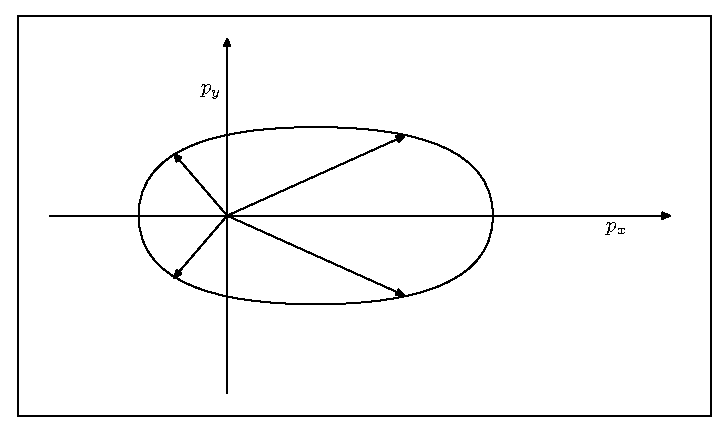
\includegraphics[height=7cm]{ellisse1.eps}
\caption{ } \label{fig:ellisse1}
\end{center}
\end{figure}

\item se $d>s_x$, l'angolo $\vartheta_{\star}$ ha un massimo,
ossia le particelle devono essere emesse in avanti, come in
f\mbox{}igura \vref{fig:ellisse2}, dove, tra l'altro, si vede
molto bene che v'\`e un angolo massimo, indicato l\`i con
$\vartheta_{\rem{max}}$, di emissione per la particella.

\begin{figure}[htbp]
\begin{center}
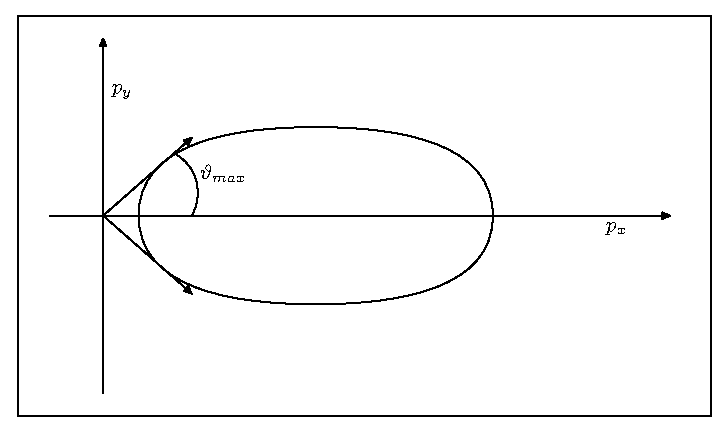
\includegraphics[height=7cm]{ellisse2.eps}
\caption{ } \label{fig:ellisse2}
\end{center}
\end{figure}
\end{enumerate}
Andando ad analizzare pi\`u in profondit\`a la situazione, si
constata che se $v_{\alpha}^{\star}<v\;$\footnote{si confronti la
\ref{eq:beta}}, siamo nella prima situazione, altrimenti se
$v_{\alpha}^{\star}=0$ siamo nella seconda. \newline Per trovare
l'angolo massimo nel sistema laboratorio, mettiamo a sistema
l'equazione dell'ellisse con quella di una retta passante per
l'origine; il sistema uscente \`e:
$$
\left\{\begin{array}{l} (1-\beta)^2(p_{\alpha x}-d)^2+p^2_{\alpha
y}=p_{\star}^2\\
\left.\begin{array}{l}
p_{\alpha x}=q\cos\vartheta\\
p_{\alpha y}=q\sin\vartheta\\
\end{array}\right\}\mbox{ la pendenza \`e }\tan\vartheta\end{array}\right.
$$
Introduciamo delle quantit\`a per semplif\mbox{}icare i conti: sia
$\varepsilon'=\frac{\beta E^{\star}_{\alpha}}{c}$, da cui
$d=\varepsilon'\gamma$. Allora:
$$
(1-\beta^2)[q^2\cos^2\vartheta-2q\cos\vartheta\varepsilon'\gamma +
(\varepsilon'\gamma)^2] + q^2\sin^2\vartheta
 = p^2_{\star}
$$
Le condizioni di tangenza si hanno quando il discriminante in $q$
\`e uguale a 0. Ovvero se scriviamo $aq^2+2bq+c=0$, deve valere la
relazione $b^2-ac=0$, che \`e la condizione di annullamento del
discriminante. Lasciando al lettore questi noiosi, ma facili,
conti, scriviamo soltanto i risultati:
$$
\cos^2\vartheta_{\rem{max}}=\frac{\varepsilon'^2-p_{\star}^2}{\varepsilon'^2-
\beta^2 
p_{\star}^2}
$$

da cui
$$
\sin^2\vartheta_{\rem{max}}=\frac{p_{\star}^2(1-\beta^2)}{\varepsilon'^2-
\beta^2  
p_{\star}^2}
$$
Possiamo inf\mbox{}ine scrivere, ricordando che
$m_{\alpha}^2c^2=\left[\left(\frac{E_{\alpha}^{\star}}{c}\right)^2
- p_{\star}^2\right]$,
$$
\sin\vartheta_{\rem{max}}=\frac{p_{\star}\sqrt{(1-\beta^2)}}{\beta
m_{\alpha }\,c}.
$$
\subsection{ Distribuzione di probabilit\`a nel
decadimento} Sopra abbiamo analizzato il decadimento di una
particella, la quale ''decade'', generando due nuove particelle.
Questo fenomeno avviene per la gran parte delle particelle, quindi
\`e naturale che esso abbia molta importanza nella nostra
trattazione; tuttavia il tempo che queste particelle impegano a
decadere non \`e prevedibile, ed \`e possibile parlarne solo come
tempo medio. Ci\`o implica che \`e necessario trattare il
decadimento dal punto di vista statistico. Per esempio, se prendo
un campione di $N$ particelle $X$, dove $X$ \`e una particella che
ha tempo di decadimento $\tau$ \footnote{\hspace{0.1cm} $\tau$ \`e
da noi definito come il tempo dopo il quale le particelle $X$ non
decadute sono $\frac{N}{e}$, e non pi\`u $N$}, dopo una frazione,
che a noi non interessa meglio definire, di $\tau$, ci sono
particelle gi\`a decadute. E dopo un multiplo di $\tau$, ci
saranno particelle che dovranno ancora decadere. Quindi per un
piccolo insieme di particelle non \`e vero che il tempo di
decadimento \`e $\tau$: questo non toglie che dopo un tempo
$\tau$, \emph{in media}, le particelle di tipo $X$ siano
$\frac{N}{e}$\footnote{L'ideale sarebbe un insieme di particelle
numerabile, ma ci\`o in pratica non pu\`o accadere}.
\newline
Trattiamo ora l'argomento con maggiore precisione: prendiamo, come
prima, $N$ particelle $X$, e definiamo $N_t$ com il numero di
particelle all'istante $t$. La legge dei decadimenti \`e:
$$
\frac{\de N_t}{\de t}=-\frac{N_t}{\tau}.
$$
La sua soluzione \`e:
\begin{equation}
N_t=N_0\,e^{-\frac{t}{\tau}} \label{eq:soluzdecad}\end{equation}
Dalla (\ref{eq:soluzdecad}) si capisce un po' pi\`u chiaramente
quanto sopra detto.
\newline
Ci chiediamo ora quale sia la distribuzione di energia
\index{energia!distribuzione di} nel decadimento. Supponiamo di
avere $N$ particelle che decadono. Una frazione di loro, diciamo
$\de N$ avr\`a energia compresa tra $E$, ed $E + \de E$. Poniamo:
\begin{eqnarray*}
\frac{\de N}{N}&=&\de \chi (E)\\ \rho (E)&=&\frac{\de \chi
(E)}{\de E} \quad\mbox{\footnotesize(\`E la densit\`a di
probabilit\`a)}
\end{eqnarray*}
Nel sistema di riferimento $\cem$, la distribuzione di energia \`e
isotropa; dunque dopo aver ivi trovato le quantit\`a a cui siamo
interessati, trasformiamo i risultati; in questa trasformazione
entra in gioco l'energia nel sistema $\lab$.
\newline


\begin{figure}[htbp]
\begin{center}
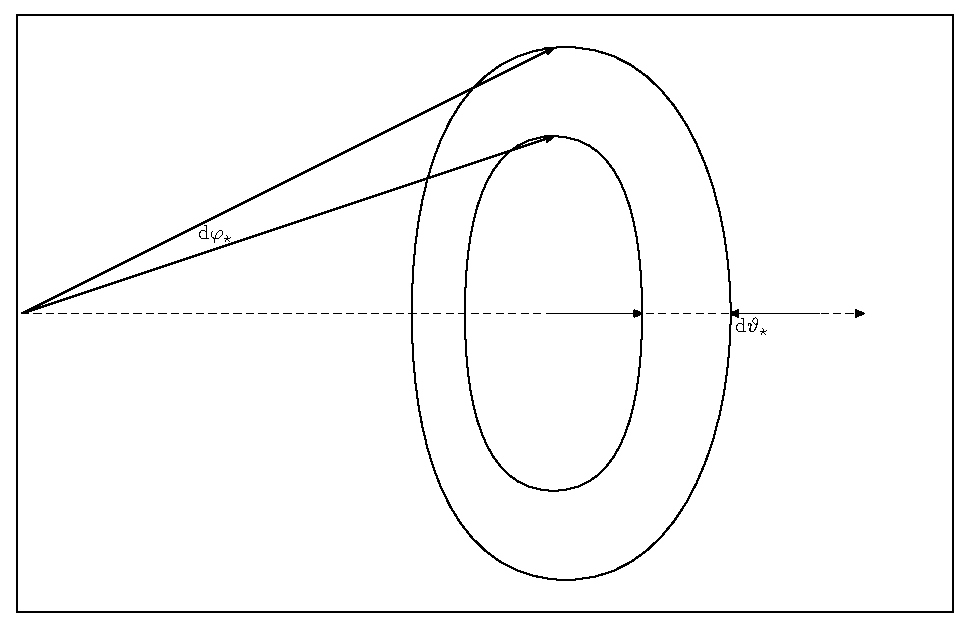
\includegraphics[height=6cm]{sezioneangolo.eps}
\caption{Sezione d'angolo solido \(\de \varphi\) e \(\de \vartheta\)
 sono invertiti rispetto alla figura} \label{fig:sezangolo}
\end{center}
\end{figure}

Con riferimento alla figura \vref{fig:sezangolo}, in $\cem$, la
probabilit\`a di trovare ua particella nell'angolo solido tra
$(\varphi^{\star},\varphi^{\star}+\de \varphi^{\star})$ e
$(\vartheta^{\star},\vartheta^{\star}+\de \vartheta^{\star})$ sono
indipendenti da $\varphi^{\star}$ e da $\vartheta^{\star}$
$$
\Longrightarrow \; \de \chi
(\varphi^{\star},\vartheta^{\star})=\frac{\de
\Omega(\varphi^{\star},\vartheta^{\star})}{4 \pi}.
$$
Per l'invarianza per rotazioni attorno all'asse $x$ si ha:
$$
\de \chi (\vartheta^{\star})=\int_{0}^{2 \pi}\frac{\de
\varphi^{\star} \;\de \cos \vartheta^{\star}}{4 \pi}=\frac{1}{2}
\de (\cos \vartheta^{\star})
$$
\`E poi cosa nota che:
\begin{equation}
E=(E^{\star}+c\beta p^{\star}\cos\vartheta^{\star})\gamma
\Longrightarrow \cos\vartheta^{\star}=\frac{E \sq
-E^{\star}}{c\beta p^{\star}} \label{eq:energiadeca}\end{equation}
da cui si ricava:
$$
\de \chi (E)=\frac{1}{2} \de (\frac{E \sq -E^{\star}}{c\beta
p^{\star}})=\frac{\de E}{2 c \beta p^{\star}\gamma}.
$$
Perci\`o in definitiva:
$$
\rho (E)=\frac{\de \chi (E)}{\de E}=\frac{1}{2}\frac{\sq}{c \beta
p_{\star}}
$$
Imponiamo in ultima le condizioni di normalizzazione:
$$
\int_{E_{\rem{min}}}^{E_{\rem{max}}} \rho (E)\,\de E=1:
\quad\mbox{ \`e una condizione plausibile?}
$$
Verifichiamolo:
\begin{equation}
\int_{E_{\rem{min}}}^{E_{\rem{max}}} \rho (E)\,\de E = \frac{1}{2 c
 \beta  p^{\star}\gamma}\,(E_{\rem{max}}-E_{\rem{min}})
\label{eq:distro}
\end{equation}
Ma, dalla (\ref{eq:energiadeca}), si ha:
$$
E_{\rem{max}}=(E^{\star}+c\beta p^{\star})\gamma
$$
ed:
$$
E_{\rem{min}}=(E^{\star}-c\beta p^{\star})\gamma
$$
da cui si ottiene che la (\ref{eq:distro}) diviene:
$$
\frac{1}{2}\frac{\sq}{c\beta p^{\star}}\gamma \,2 \,c \,\beta\,
p^{\star}=1,
$$
il che ci permette di concludere questa parte.
\subsection{ Urti tra particelle}
\footnote{ Usiamo la convenzione $c=1$} Per quanto rigurda i
processi d'urto tra particelle, nella nostra analisi, prenderemo
in considerazione solo urti elastici, ovvero urti dove le
particelle uscenti sono dello stesso tipo di quelle entranti. Per
focalizzare come avviene il processo d'urto tra due particelle,
possiamo riferirci alla figura \vref{fig:urto}.

\begin{figure}[htbp]
\begin{center}
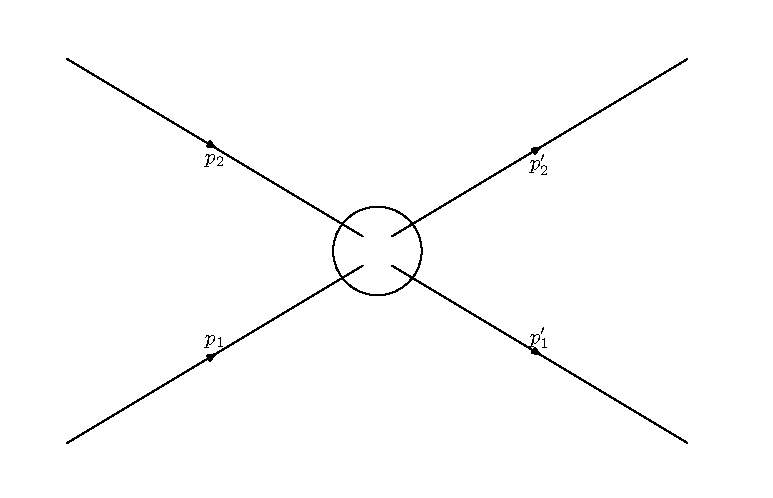
\includegraphics[width=10cm]{urto.eps}
\caption{Figura d'un urto elastico} \label{fig:urto}
\end{center}
\end{figure}

Quanti invarianti relativistici possiamo avere con tale processo?
Sappiamo che vale la conservazione del quadrimpulso, cio\`e che:
$$
p_1+p_2=p'_1+p'_2,
$$
il che implica:
$$
E_1+E_2=E'_1+E'_2, \quad\mbox{ un'equazione,}
$$
e
$$
\mathbf{p}_1+\mathbf{p}_2=\mathbf{p}_1{}'+\mathbf{p}_2{}',
\quad\mbox{ tre equazioni;}
$$
Inoltre abbiamo
$p_{{}_{1,2}}^2=m_{{}_{1,2}}^2=(p'_{{}_{1,2}}{})^2$, ovvero altre
quattro equazioni. Abbiamo dunque 8 condizioni sui sedici
parametri che compongono i 4 quadrimpulsi. Quindi si hanno altri 8
parametri liberi, che tuttavia scendono a due poich\`e possiamo
scegliere, mediante una rotazione e una trasformazione di Lorentz,
il sistema di riferimento che ci \`e pi\`u congeniale (e tale
operazione porta via altri 6 parametri). Vedremo pi\`u avanti cosa
rappresentano questi 2 parametri liberi.
\subsection{ Le variabili di Mandelstam}
\footnote{ Usiamo la convenzione $c=1$}
\index{Mandelstam!variabili di}Nello studio relativistico degli
urti tra particelle, sono state introdotte, da Mandelstam, quattro
invarianti relativistici, cos\`i definiti\footnote{\(s\) \`e anche detto
massa invariante, mentre \(t\) \`e anche detto momento invariante.}:
$$
s=(p_1+p_2)^2=(p'_1+p'_2)^2
$$
$$
t=(p_1-p'_1)^2=(p_2-p'_2)^2
$$
$$
u=(p_1-p'_2)^2=(p_2-p'_1)^2
$$
\begin{equation}
s+t+u=2(m_1^2+m_2^2). \label{eq:mandelstam}
\end{equation}
Non \`e difficile verificare la (\ref{eq:mandelstam}); infatti:
\begin{eqnarray*}
s+t+u & = & (p_1+p_2)^2+(p_1-p'_1)^2+(p_1-p'_2)^2\\ & =  & 3 p_1^2
+ p_2^2 + p'_1{}^2+p'_2{}^2 - 2 p_1 (p'_1 + p'_2 - p_2)
\end{eqnarray*}
dalla quale, ricordando che $p_1 + p_2 = p'_1 + p'_2$, e che
$p_i^2 = m_i^2$, si ottiene la (\ref{eq:mandelstam}). \newline
Possiamo ora specificare il dominio fisico di $s$, che risulta
essere $s\in[(m_1+m_2)^2,\infty]$; lo si verifica non troppo
difficilmente:
\begin{eqnarray*}
s & = & (p_1+p_2)^2\\
  & = & (p_1^{\star}+p_2^{\star})^2\\
  & \stackrel{\bigstar}{=} & (E_1^{\star}+E_2^{\star})^2\\
  & = & (\sqrt{p_{\star}^2 + m_1^2} + \sqrt{p_{\star}^2 +
  m_2^2})^2\\
  & \geq & (m_1 + m_2)^2
\end{eqnarray*}
L'unico passaggio che potrebbe necessitare delucidazioni \`e
$\bigstar$: chiariamo subito: nel CM valgono le relazioni:
\begin{equation}\left\{\begin{array}{ccc}
p_1^{\star} = (E_1^{\star},p^{\star},0,0)\\
p_2^{\star} = (E_2^{\star},-p^{\star},0,0)
\end{array}\right.\Longrightarrow |p_1^{\star} + p_2^{\star}| =
E_1^{\star} + E_2^{\star} \label{eq:abcd}
\end{equation}
e questo pu\`o essere sufficiente, a mio parere, per la
spiegazione.
\newline
Scriviamo poi un'altra relazione che ci torner\`a utile, tra le
altre cose, per la caratterizzazione del dominio fisico di $t$;
per la conservazione di $p$ si ha (nel caso di due particelle che
si urtano):
$$
\mathbf{p}_1^{\star} + \mathbf{p}_2^{\star}=\mathbf{p}_1^{'\star}
+ \mathbf{p}_2^{'\star}=\mathbf{0}
$$
$$
\Longrightarrow
$$
$$
p_{\star}=|\mathbf{p_{1}^{\star}}|=|\mathbf{p_{2}^{\star}}| \quad
\& \quad
p'_{\star}=|\mathbf{p_{1}^{'\star}}|=|\mathbf{p_{2}^{'\star}}|;
$$
Applicando la conservazione dell'energia:
$$
E_1^{\star} + E_2^{\star} = E_1^{'\star} + E_2^{'\star}
$$
$$
\Longrightarrow
$$
$$
\sqrt{p_{\star}^2 + m_1^2} + \sqrt{p_{\star}^2 +
  m_2^2} = \sqrt{p_{\star}^{'2} + m_1^2} + \sqrt{p_{\star}^{'2} +
  m_2^2}
$$
Tale relazione vale $\Leftrightarrow$ $p_{\star}=p'_{\star}$.
Ci\`o implica che:
$$
|\mathbf{p_{1}^{\star}}| = |\mathbf{p_{2}^{\star}}| =
|\mathbf{p_{1}^{'\star}}| = |\mathbf{p_{2}^{'\star}}| = p_{\star}
$$
Possiamo a questo punto caratterizzare $t$:
$$
t = (p'_1-p_1)^2 = (E_1^{'\star} - E_1^{\star})^2 -
(\mathbf{p}_1^{'\star} - \mathbf{p}_1^{\star})^2 =
$$
$$
0 - 2 p_{\star}^2(1 - \cos \vartheta_{\star}) \leq 0 \quad
(\rem{infatti }\;\; E_1^{'\star} = \sqrt{m_1^2 +
p_{\star}^2}=E_1^{\star}, \rem{ e }
p'_1=p^{\star}\cos\vartheta^{\star})
$$
Da queste due caratterizzazioni e da $ s + t + u = 2 (m_1^2 +
m_2^2)$, ne esce che l'intervallo fisico di $u$ \`e determinato da
$m_1$ ed $m_2$.
\subsection{ Gli urti veri e propri}
\footnote{ Usiamo la convenzione $c=1$} Ora che abbiamo introdotto
le variabili di Mandelstam, siamo in possesso di invarianti utili
alla formalizzazione del processo di urti tra particelle.
Prendiamo in considerazione l'urto in figura \vref{fig:urto}, tra
la particella 1, che, prima dell'urto, in $\lab$, ha quadrimpulso
pari a:
$$
p_1=(E_1,\mathbf{p}_1)
$$
e la particella 2, ferma in $\lab$, e che dunque ha quadrimpulso:
$$
p_2=(m_2,\mathbf{0}).
$$
Indichiamo con l'apice le quantit\`a dopo l'urto, e senz'apice le
quantit\`a prima dell'urto. La conservazione dell'energia in
$\lab$ implica:
\begin{equation}
E_1 + m_2 = E'_1 + E'_2 \longrightarrow E'_1 - E_1 = m_2 - E'_2.
\label{eq:energia_urto}
\end{equation}
Calcoliamoci gli invarianti relativistici:
\footnote{Ricordarsi che $p_i^2 = m_i^2$}
\begin{eqnarray*}
s_{\lab} &=& m_1^2 + m_2^2 + 2 (E_1 E_2 - \mathbf{p_1}\mathbf{p_2})\\
& \stackrel{E_2 = m_2,\;\; \mathbf{p_2}=\mathbf{0}}{=} & m_1^2 +
m_2^2 + 2 m_2 E_1
\end{eqnarray*}
\begin{eqnarray*}
t_{\lab} & = &  (p'_1-p_1)^2 \\ & = & (p'_2-p_2)^2  \\ & = & 2
m_2^2 -2 (E'_2 E_2 - \mathbf{p'_2}\mathbf{p_2})  \\ & \stackrel{
E_2 = m_2,\;\;\mathbf{p_2} = \mathbf{0} }{=} & 2 m_2^2 - m_2 E'_2 \\
& = & 2 m_2 (m_2 - E'_2) \\ &
\stackrel{(\ref{eq:energia_urto})}{=} & 2 m_2 (E'_1 - E_1).
\end{eqnarray*}
Ora sfruttiamo il fatto che $s_{\lab}=s_{\cem}$, ottenendo
(ricorda (\ref{eq:abcd})):
$$
\left(\sqrt{p_{\star}^2 + m_1^2} + \sqrt{p_{\star}^2 +
m_2^2}\right)^2 = m_1^2 + m_2^2 + 2 m_2 E_1
$$
$$
p_{\star}^2 + m_1^2 + p_{\star}^2 + m_2^2 + 2 \sqrt{p_{\star}^2 +
m_1^2}  \sqrt{p_{\star}^2 + m_2^2} = m_1^2 + m_2^2 + 2 m_2 E_1
$$
Semplificando:
$$
\sqrt{p_{\star}^2 + m_1^2}  \sqrt{p_{\star}^2 + m_2^2} = ( m_2 E_1
- p_{\star}^2)
$$
Elevando al quadrato otteniamo:
$$
p_{\star}^4 + p_{\star}^2 (m_1^2 + m_2^2) + m_1^2  m_2^2 = m_2^2
E_1^2 + p_{\star}^4 - 2 p_{\star}^2 m_2 E_1
$$
$$ p_{\star}^2 = \frac{m_2^2 (E_1^2 - m_1^2)}{m_1^2 + m_2^2 + 2
m_2 E_1}:
$$
$$\quad\mbox{\textsc{ho trovato} } p_{\star} \mbox{ \textsc{in funzione di
}} E_1.
$$
Vale poi $t_{\lab}=t_{\cem}$, ovvero:
$$
-2 p_{\star}^2 (1 - \cos\vartheta^{\star}) = 2 m_2 (E'_1 - E_1)
$$
$$
\Longrightarrow
$$
\begin{eqnarray*}
E'_1 & = & -\frac{2 p_{\star}^2}{2 m_2} (1-\cos \vartheta_{\star})
+ E_1\\
& = & -\frac{ p_{\star}^2}{ m_2} (1-\cos \vartheta_{\star}) + E_1\\
\end{eqnarray*}
Ora anche $E'_1$ \`e noto in funzione di $E_1$ e
$\vartheta_{\star}$. A questo punto $E'_{1_{max}}$ ed
$E'_{1_{min}}$ si ricavano facilmente. $E'_{1_{max}}= E'_1(\cos
\vartheta_{\star} = 1)$, e dunque $E'_{1_{max}}= E_1$. Invece:
$$
E'_{1_{min}} = \frac{E_1 (m_1^2 + m_2^2) + 2 m_2 m_1^2}{m_1^2 +
m_2^2 + 2 E_1 m_2}.
$$
\begin{observazione}
In fisica relativistica \`e possibile trasferire energia, anche in
quantit\`a molto grande, da una massa $m_1<<m_2$, alla massa
$m_2$, cosa che non era prevista prima. Infatti, nella condizione
$m_1<<m_2$:
$$
\frac{E'_{k\,\rem{min}_1}}{E_{k\,\rem{min}_1}}
\stackrel{m_1<<m_2}{\longrightarrow} \frac{m_2}{m_2 + E_1}
\stackrel{E_1 \rightarrow \infty}{\longrightarrow} 0.
$$
In fisica non relativistica invece $E - m \approx m v^2 / 2$,
$v^2<<c^2$ e perci\`o $E_1 m_2 \approx m_1 m_2$. Allora:
$$
\frac{E'_{k\,\rem{min}_1}}{E_{k\,\rem{min}_1}} \stackrel{v/c
<<1}{\approx} \frac{(m_1-m_2)^2}{m_1 + m_2} \stackrel{m_1 <<
m_2}{\longrightarrow} 1,
$$
come si voleva mostrare.
\end{observazione}
Se ora vogliamo stabilire come si dispongono gli impulsi dopo
l'urto, si procede analogamente a come proceduto nel decadimento,
sapendo il risultato della somma vettoriale $\mathbf{p'_1} +
\mathbf{p'_2} = \mathbf{p_1}$.
\newline
Ne esce dunque l'equazione dell'ellisse:
$$
\frac{ (p'_{y\,\alpha})^2 }{ p_{\star}^2 } + \frac{ 1- \beta^2 }{
p_{\star}^2 } \left( p'_{x\,\alpha} - \frac{ \beta
E_{\alpha}^{\star} }{ \sqrt{ 1 - \beta^2} }\right)^2 = 1.
$$
Si lascia al lettore farsi i vari casi, come nel decadimento.







%
